\documentclass[../talk.tex]{subfiles}
\begin{document}

\begin{frame}{Automata theory}
    \begin{overlayarea}{\slidewidth}{\slideheight}
        \alert{Verification problem}

        \begin{problem}
            \problemtitle{Verification problem for specification $\varphi$}
            \probleminput{Program $P$.}
            \problemquestion{Does behavior of $P$ satisfy $\varphi$, $P \models \varphi$?}
        \end{problem}

        \sonslide<2->%
        {%
            \alert{Automated verification:}
            \begin{center}
                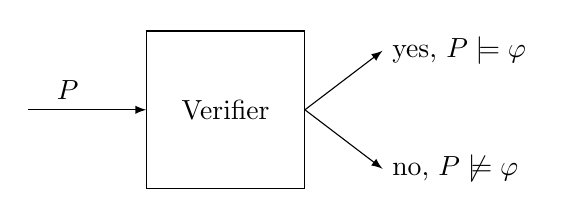
\begin{tikzpicture}
                    \node (origin) [coordinate] at (0.5,0) {};
                    \node (rect) at (2,0) [minimum width=2cm,minimum height=2cm, anchor=west,draw] {};
                    \node (yes) [coordinate] at (5,0.75) {};
                    \node (no) [coordinate] at (5,-0.75) {};
                    \path [->,>=latex]
                        (origin) edge (rect.west)
                        (rect.east) edge (yes)
                        (rect.east) edge (no)
                    ;

                    \node at (1,0.25) {$P$};
                    \node [right of=yes, node distance=0cm, anchor=west] {yes, $P \models \varphi$};
                    \node [right of=no, node distance=0cm, anchor=west] {no, $P \not\models \varphi$};
                    \node at (rect) {Verifier};
                \end{tikzpicture}
            \end{center}
        }
        \ifshowfull%
            \only<3>%
            {%
                \begin{theorem}[{[Church 1935/36, Turing 1936]}]
                    The verification problem is undecidable for \alert{some} specification.
                \end{theorem}
            }
        \fi%
        \sonslide<4->%
        {%
            \begin{theorem}[{[Church 1935/36, Turing 1936, Rice 1953]}]
                The verification problem is undecidable for \alert{all} specifications.
            \end{theorem}
        }
    \end{overlayarea}
\end{frame}

\end{document}
